% Lesson: why a cached TikZ figure drawn with flags comes out wrong, and how to name it.
% Compile with:  latexmk  (settings in .latexmkrc)

\documentclass[11pt,a4paper]{article}

\usepackage{fontspec}
\usepackage[margin=2.2cm]{geometry}
\usepackage{xcolor}
\usepackage[most]{tcolorbox}
\usepackage{listings}
\usepackage{twemojis}
\usepackage{lesson}
\usepackage{enumitem}
\usepackage{booktabs}
\usepackage{needspace}
\usepackage{graphicx}
\usepackage[colorlinks=true,linkcolor=blue!50!black,urlcolor=blue!50!black,citecolor=blue!50!black]{hyperref}
\usepackage[capitalise,nameinlink]{cleveref}
\usepackage{newunicodechar}
\newunicodechar{→}{\ensuremath{\rightarrow}}

\newif\ifRed  % the demo's flag, for the preview

\setlength{\parindent}{0pt}
\setlength{\parskip}{0.6em}
\setlength{\emergencystretch}{3em}

\renewcommand{\panetitle}{A terminal on \name{AlfMAC4}, in \name{demo/}}

% This lesson's panes and outputs are short: keep each whole on one page, instead of
% lesson.sty's breakable boxes, which can leave a frame split across a page break
\renewtcblisting{pane}{listing engine=listings, listing only, enhanced, unbreakable,
  colback=blue!12, colframe=blue!70!black, boxrule=0.6pt, arc=2pt,
  colbacktitle=blue!60, coltitle=black, title={\emo{desktop computer}\ \panetitle}, fonttitle=\small\bfseries,
  listing options={style=shell}}
\renewtcblisting{cmdout}{listing engine=listings, listing only, enhanced, unbreakable,
  colback=white, colframe=black!25, boxrule=0.4pt, arc=1pt, left=4pt,
  title={Output}, fonttitle=\scriptsize, coltitle=black!70, colbacktitle=black!6,
  listing options={style=out}}

% A source file shown whole: start it on the next page unless eight lines are left
\let\lstinputlistingwhole\lstinputlisting
\renewcommand{\lstinputlisting}[2][]{\needspace{8\baselineskip}\lstinputlistingwhole[#1]{#2}}
% A command and its output travel together: start the pane on the next page unless
% fourteen lines are left
\BeforeBeginEnvironment{pane}{\needspace{14\baselineskip}}
% A heading travels with its snippet: start it on the next page unless eight lines are left
\let\sectionalone\section
\renewcommand{\section}{\needspace{8\baselineskip}\sectionalone}

% A single control sequence in prose, e.g. \cs{edef}
\newcommand{\cs}[1]{\texttt{\textbackslash #1}}
% The demo's \fig, coloured as in the listings
\newcommand{\fig}{\texttt{\color{magenta!75!black}\textbackslash fig}}
% A named flag in prose, split and coloured as in the listings: \flagif{Red}, \flagtrue{Red}
\newcommand{\flagif}[1]{\texttt{\lstflagif{#1}{}}}
\newcommand{\flagtrue}[1]{\texttt{\lstflagtrue{#1}{}}}

% A named flag in two colours, \if and true orange, the flag's own name teal. listings reads
% \ifReLU as one control word and hands it to the style as #2: ignore it, print the split
\newcommand{\lstflagif}[2]{{\color{orange!85!black}\textbackslash if}{\color{teal!80!black}#1}}
\newcommand{\lstflagtrue}[2]{{\color{teal!80!black}\textbackslash #1}{\color{orange!85!black}true}}

% A LaTeX source file, shown as it is
% Colours: naming commands blue, \if \else \fi orange (a flag's own name teal), drawing commands
% violet, the rest grey; braces green, so the names inside them stand out
\lstdefinestyle{latex}{style=out, language=[LaTeX]TeX, basicstyle=\ttfamily\footnotesize\color{black!85},
  frame=single, rulecolor=\color{black!25}, framesep=5pt, xleftmargin=5pt, xrightmargin=5pt,  % a border, no fill
  texcsstyle=*\color{black!55},
  % The LaTeX language already lists primitives such as \else, \fi, \input in its first
  % class, which wins: remove them there, so the classes below can claim them
  deletetexcs={else,fi,if,input,def,edef,gdef,begin,end,hskip,fill,newif,documentclass,usepackage},
  moretexcs=[2]{tikzsetnextfilename,tikzset,tikzexternalize,edef,def,gdef,circlename},
  texcsstyle=*[2]\color{blue!75!black},
  moretexcs=[3]{if,else,fi,newif},
  texcsstyle=*[3]\color{orange!85!black},
  moretexcs=[4]{fill,begin,end,input,usepackage,usetikzlibrary,documentclass,pdfcompresslevel,hskip},
  texcsstyle=*[4]\color{violet!80!black},
  commentstyle=\color{black!40}\itshape,
  % listings treats TeX primitives (\else, \fi, \input, \def, …) as keywords, not as
  % control sequences: drop them from the keywords so the groups above colour them
  deletekeywords={else,fi,if,input,def,edef,gdef,begin,end,hskip,fill,newif},
  % One class per named flag, each printing its own split
  moretexcs=[6]{ifRed}, texcsstyle=*[6]\lstflagif{Red},
  moretexcs=[7]{Redtrue}, texcsstyle=*[7]\lstflagtrue{Red},
  moretexcs=[8]{ifReLU}, texcsstyle=*[8]\lstflagif{ReLU},
  moretexcs=[9]{ReLUtrue}, texcsstyle=*[9]\lstflagtrue{ReLU},
  moretexcs=[10]{ifTanh}, texcsstyle=*[10]\lstflagif{Tanh},
  moretexcs=[11]{Tanhtrue}, texcsstyle=*[11]\lstflagtrue{Tanh},
  moretexcs=[12]{ifSigmoid}, texcsstyle=*[12]\lstflagif{Sigmoid},
  moretexcs=[13]{Sigmoidtrue}, texcsstyle=*[13]\lstflagtrue{Sigmoid},
  moretexcs=[14]{ifModelManifold}, texcsstyle=*[14]\lstflagif{ModelManifold},
  moretexcs=[15]{ifUenergy}, texcsstyle=*[15]\lstflagif{Uenergy},
  moretexcs=[16]{fig}, texcsstyle=*[16]\color{magenta!75!black},  % the experiment's name
  literate={\{}{{\color{green!45!black}\{}}1 {\}}{{\color{green!45!black}\}}}1}

\newtcolorbox{result}[1]{enhanced, breakable, colback=green!22, colframe=green!50!black,
  colbacktitle=green!60, coltitle=black, title={\emo{check mark button}\ #1}, fonttitle=\bfseries, boxrule=1pt, arc=2pt}

\title{\emo{framed picture}\ One figure file, several cached pictures\\[0.3em]
  \large TikZ caches by name and source text, not by flag, so each variant needs its own name}
\author{Lesson for Alfredo Canziani, written by Claude}
\date{Thu 29 Oct 2026}

\begin{document}
\maketitle

\section*{Why we asked}

Several figure files in the book are drawn more than once, each time with a different flag switched on first: \name{inference-figs/activation.tex} (ReLU, tanh, sigmoid), \name{inference-figs/scatter.tex}, \name{ellipse-figs/ellipse.tex}, and \name{spiral-figs/ambient-space.tex}. In \name{inference.tex}, for example:

\begin{lstlisting}[style=latex]
{\ReLUtrue\input{inference-figs/activation}}\hskip 10pt
{\Tanhtrue\input{inference-figs/activation}}\hskip 10pt
{\Sigmoidtrue\input{inference-figs/activation}}%
\end{lstlisting}

My convention gives every variant its own \emph{literal} name, picked by the flags, in one of two ways. The first is an \cs{if}…\cs{else} chain, as at the top of \name{activation.tex} (and \name{scatter.tex}):

\begin{lstlisting}[style=latex]
\ifReLU\tikzsetnextfilename{inference-ReLU}
\else\ifTanh\tikzsetnextfilename{inference-Tanh}
\else\ifSigmoid\tikzsetnextfilename{inference-Sigmoid}\fi\fi\fi
\end{lstlisting}

The second is a default name, then one line per flag that overrides it, as at the top of \name{ellipse.tex}:

\begin{lstlisting}[style=latex]
\tikzsetnextfilename{ellipse-ambient-space}
\ifModelManifold\tikzsetnextfilename{ellipse-ambient-space-and-manifold}\fi
\ifUenergy\tikzsetnextfilename{ellipse-ambient-space-and-manifold-U-annotated}\fi
\end{lstlisting}

\name{ambient-space.tex} was the exception. Until 23 May 2022 the spiral figure was a PDF made in Python, \name{python/spiral-figs/test.pdf}. Commit \texttt{85edb9f}, \textit{Replace spiral PDF with TikZ}, redrew it in TikZ and cached it under one name, which was right at the time: the file drew one picture.

\begin{lstlisting}[style=latex]
\tikzsetnextfilename{spiral-ambient-space}
%\tikzset{external/export next=false}
\end{lstlisting}

On 8 Jun 2022, commit \texttt{24a37ac}, \textit{Add trained model figures}, added the first flags (\flagif{LinearModel}, \flagif{NonlinearModel}, \flagif{VectorField}, \flagif{Embedding}) and, in the same commit, swapped those two lines. From then on the file had caching switched off, so its \name{pgfplots} panels were redrawn on every build, which is why the spiral chapter compiled slowly:

\begin{lstlisting}[style=latex]
%\tikzsetnextfilename{spiral-ambient-space}
\tikzset{external/export next=false}
\end{lstlisting}

The override form was already in the book: \name{ellipse.tex} got it on 20 May 2022, nineteen days earlier (commit \texttt{fcc8d42}, \textit{Add conditional names to figure, remove underscores}). The commit message of \texttt{24a37ac} lists the four new figures only.

Today the spiral chapter compiled slowly, Claude found the switch, and I asked it to toggle the comment: caching on again, under the one fixed name \texttt{spiral-ambient-space}. Later, after the training-data figure moved to the chapter opening, I asked Claude to regenerate it. Claude listed the cache folder, \name{build/pdf-tikz-figs/}, and found a single \name{spiral-ambient-space.pdf} for a file that \name{spiral.tex} inputs seven times, six of them with a flag on. One name means one cached picture, so every variant showed the same image. Claude read this off the file list, before opening any PDF; \Cref{sec:fixed} reproduces it. Then, instead of following my convention, Claude named the variants with an \cs{edef} (\Cref{sec:edef}) that builds the name from the flags. I asked why that \cs{edef} is needed.

To answer, we rebuilt the situation in miniature, in \name{demo/}. \Cref{sec:demo} shows it, after a look at what externalisation does.

\section{What externalisation does}

\begin{insight}{Externalisation}
With \cs{tikzexternalize}, every \texttt{tikzpicture} is compiled once, on its own, into a small PDF; the document then includes that PDF instead of redrawing the picture. Two things identify the cached file:
\begin{itemize}[leftmargin=1.2em,itemsep=0pt]
  \item its \textbf{name}, set by \cs{tikzsetnextfilename}, which is also the file name on disk;
  \item a \textbf{fingerprint} (an MD5 sum) of the picture's \emph{source text}, stored in a \name{.md5} file next to it. If the fingerprint matches, TikZ calls the image up to date and reuses it.
\end{itemize}
The fingerprint is taken from the code as written, before \TeX\ runs it. A flag such as \flagif{ReLU} is part of that text, but its value is not. In the manual's words, ``\,`picture content' only includes the top-level tokens; no expansion is applied'' \cite[§52.4 \textit{Externalizing graphics}, p.~676]{tikz}.
\end{insight}

\section{The demo}\label{sec:demo}

Everything is in \name{demo/}. The picture comes first:

\lstinputlisting[style=latex, title={\name{circle.tex}}]{demo/circle.tex}

\name{circle.tex} draws a filled circle: blue, or red when the flag \flagif{Red} is true.

\begin{center}
\begin{tabular}{@{}c@{\hspace{2cm}}c@{}}
  \scalebox{0.4}{
\begin{tikzpicture}
  \ifRed\fill [red] (0,0) circle (1);\else\fill [blue] (0,0) circle (1);\fi
\end{tikzpicture}
} & \scalebox{0.4}{\Redtrue
\begin{tikzpicture}
  \ifRed\fill [red] (0,0) circle (1);\else\fill [blue] (0,0) circle (1);\fi
\end{tikzpicture}
} \\[0.3em]
  \small \flagif{Red} false & \small \flagif{Red} true \\
\end{tabular}
\end{center}

The two pictures differ, so each needs its own cached image, under its own name. We tried six ways of naming them: the fixed name, no caching, my two conventions, and Claude's two variants. Each way is one experiment, made of three files. For the experiment \texttt{fixed}:
\begin{itemize}[leftmargin=1.2em,itemsep=0pt]
  \item \name{fixed.tex}, the \emph{driver}:
\lstinputlistingwhole[style=latex, title={\name{fixed.tex}}]{demo/fixed.tex}  % one line: no page-break guard
We compile it with \texttt{pdflatex -shell-escape fixed}. Its one line stores the experiment's name, \texttt{fixed}, in the macro \fig, then reads \name{main.tex}. The other five drivers differ only in the name they store: \texttt{off}, \texttt{chain}, \texttt{override}, \texttt{edef}, and \texttt{inline}.
  \item \name{main.tex}, the \emph{document}, shared by all six experiments:
\lstinputlisting[style=latex, title={\name{main.tex}}]{demo/main.tex}
Its three working lines:
  \begin{itemize}[leftmargin=1.2em,itemsep=0pt]
    \item \lstinline[style=latex, frame=none]|\tikzexternalize[prefix=figs/\fig-]| switches caching on. Every cached image goes into \name{figs/}, and its file name starts with the experiment's name and a dash.
    \item \lstinline[style=latex, frame=none]|\newif\ifRed| creates the flag, false at first.
    \item \lstinline[style=latex, frame=none]|\input{\fig-circle}| reads the figure file, here \name{fixed-circle.tex}: once as it is, then once more inside a group where \flagtrue{Red} sets the flag.
  \end{itemize}
  \item \name{fixed-circle.tex}, the \emph{figure file}:
\lstinputlistingwhole[style=latex, title={\name{fixed-circle.tex}}]{demo/fixed-circle.tex}  % two lines: no page-break guard
\cs{tikzsetnextfilename} names the next picture \texttt{circle}; with the prefix from \name{main.tex}, it is cached as \name{figs/fixed-circle.pdf}. \texttt{\textbackslash input\{circle\}} then reads \name{circle.tex}, which draws it. This is the only file that differs from one experiment to the next.
\end{itemize}

\needspace{17\baselineskip}
The chain for \texttt{fixed}, from the command to the cache:

\begin{center}
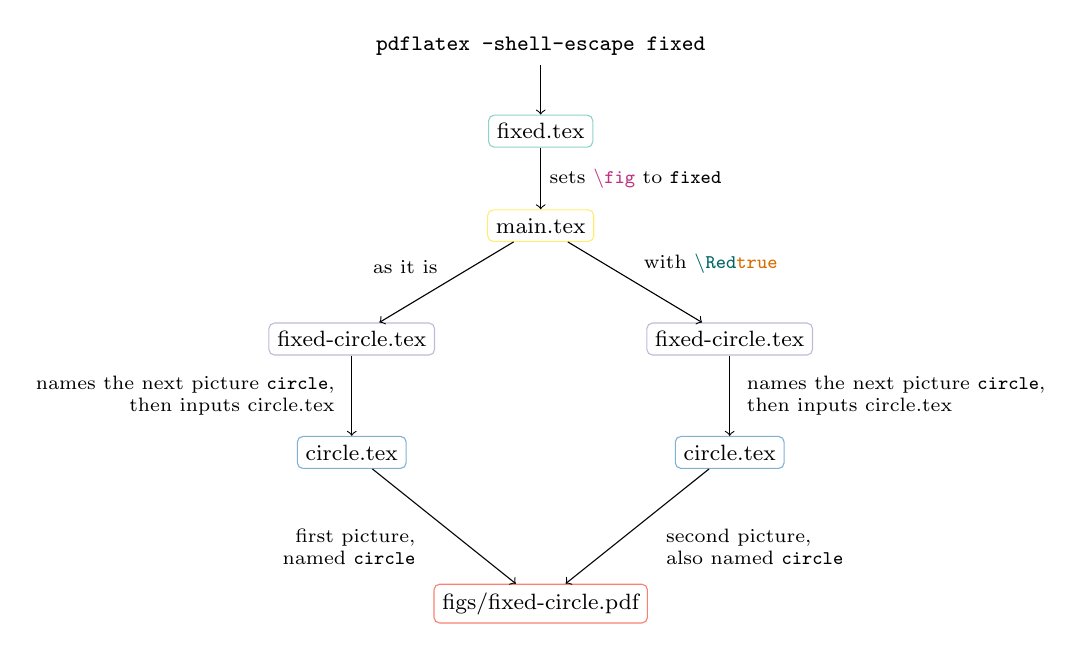
\begin{tikzpicture}[x=1cm, y=1.2cm, font=\footnotesize,
    file/.style={draw, rounded corners=2pt, inner sep=3pt},
    lab/.style={font=\scriptsize, inner sep=3pt, align=left}]
  \definecolor{drv}{HTML}{8DD3C7}\definecolor{mn}{HTML}{FFED6F}  % ColorBrewer Set3, as borders
  \definecolor{fg}{HTML}{BEBADA}\definecolor{ch}{HTML}{FB8072}\definecolor{pic}{HTML}{80B1D3}
  \node (cmd) at (0,0.9) {\texttt{pdflatex -shell-escape fixed}};
  \node[file, draw=drv] (d) at (0,0) {\name{fixed.tex}};
  \node[file, draw=mn] (m) at (0,-1) {\name{main.tex}};
  \node[file, draw=fg] (f1) at (-2.4,-2.2) {\name{fixed-circle.tex}};
  \node[file, draw=fg] (f2) at (2.4,-2.2) {\name{fixed-circle.tex}};
  \node[file, draw=pic] (c1) at (-2.4,-3.4) {\name{circle.tex}};
  \node[file, draw=pic] (c2) at (2.4,-3.4) {\name{circle.tex}};
  \node[file, draw=ch] (k) at (0,-5.0) {\name{figs/fixed-circle.pdf}};
  \draw[->] (cmd) -- (d);
  \draw[->] (d) -- node[right, lab] {sets \fig\ to \texttt{fixed}} (m);
  \draw[->] (m) -- node[above left, lab] {as it is} (f1);
  \draw[->] (m) -- node[above right, lab] {with \flagtrue{Red}} (f2);
  \draw[->] (f1) -- node[left=3pt, lab, align=right] {names the next picture \texttt{circle},\\then inputs \name{circle.tex}} (c1);
  \draw[->] (f2) -- node[right=3pt, lab] {names the next picture \texttt{circle},\\then inputs \name{circle.tex}} (c2);
  \draw[->] (c1) -- node[pos=0.4, below left=2pt, lab, align=right] {first picture,\\named \texttt{circle}} (k);
  \draw[->] (c2) -- node[pos=0.4, below right=2pt, lab] {second picture,\\also named \texttt{circle}} (k);
\end{tikzpicture}
\end{center}

Both pictures get the same name; \Cref{sec:fixed} shows what TikZ does with that.

The six experiments side by side:

\begin{center}
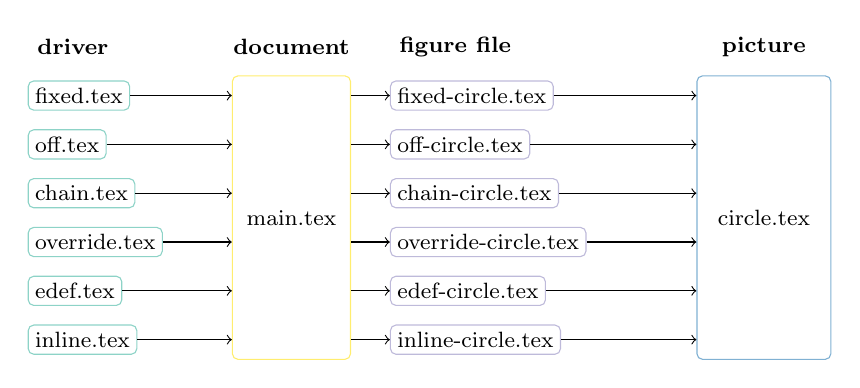
\begin{tikzpicture}[x=1cm, y=-0.62cm, font=\footnotesize,
    file/.style={draw, rounded corners=2pt, inner sep=2.5pt, anchor=west}]
  \definecolor{drv}{HTML}{8DD3C7}\definecolor{mn}{HTML}{FFED6F}  % ColorBrewer Set3, as borders
  \definecolor{fg}{HTML}{BEBADA}\definecolor{pic}{HTML}{80B1D3}
  \node[font=\footnotesize\bfseries, anchor=west] at (0,0) {driver};
  \node[font=\footnotesize\bfseries] at (3.35,0) {document};
  \node[font=\footnotesize\bfseries, anchor=west] at (4.6,0) {figure file};
  \node[font=\footnotesize\bfseries] at (9.35,0) {picture};
  \node[draw=mn, rounded corners=2pt, minimum width=1.5cm, minimum height=3.6cm]
    (m) at (3.35,3.5) {\name{main.tex}};
  \node[draw=pic, rounded corners=2pt, minimum width=1.7cm, minimum height=3.6cm]
    (c) at (9.35,3.5) {\name{circle.tex}};
  \foreach \e [count=\i] in {fixed, off, chain, override, edef, inline} {
    \node[file, draw=drv] (d\i) at (0,\i) {\name{\e.tex}};
    \node[file, draw=fg] (f\i) at (4.6,\i) {\name{\e-circle.tex}};
    \draw[->] (d\i.east) -- (d\i.east -| m.west);
    \draw[->] (f\i.west -| m.east) -- (f\i.west);
    \draw[->] (f\i.east) -- (f\i.east -| c.west);
  }
\end{tikzpicture}
\end{center}

\section{One fixed name, as in the first attempt}\label{sec:fixed}

\lstinputlisting[style=latex, title={\name{fixed-circle.tex}}]{demo/fixed-circle.tex}

\begin{pane}
$ pdflatex -shell-escape -interaction=batchmode fixed   # compile, externalising each picture
$ grep --text --only-matching --extended-regexp '(0 0 1|1 0 0) rg' fixed.pdf \
    | sort | uniq --count   # count blue and red fills
\end{pane}
\begin{cmdout}
   |!2 0 0 1 rg!|
\end{cmdout}

The first command compiles the experiment. The second counts the colours in the PDF, which fills a shape after setting its colour with \texttt{r g b rg}: \texttt{0 0 1 rg} is blue, \texttt{1 0 0 rg} is red.
\begin{itemize}[leftmargin=1.2em,itemsep=0pt]
  \item \texttt{grep --text} reads the PDF as text; \texttt{--only-matching} prints only the matched part, one match per line; \texttt{--extended-regexp} lets \texttt{|} mean \emph{or}.
  \item \texttt{sort} puts identical lines next to each other.
  \item \texttt{uniq --count} merges each run of identical lines into one, and prints the line after how many there were: \texttt{2 0 0 1 rg} is \texttt{0 0 1 rg} twice.
\end{itemize}

Two blue circles, no red one. The log says why:

\begin{pane}
$ grep --line-number 'figs/fixed-circle' fixed.log   # what TikZ did with figs/fixed-circle
\end{pane}
\begin{cmdout}
|~398:\openout3 = `figs/fixed-circle.md5'.~|
|~403:n-error -interaction=batchmode -jobname "figs/fixed-circle" "\def\tikzexternalr~|
406: "figs/fixed-circle" "\def\tikzexternalrealjob{fixed}\input{fixed}")...executed
|!412:===== Image 'figs/fixed-circle' is up-to-date. ======!|
|~416:fixed-circle.pdf> <./figs/fixed-circle.pdf>] (./fixed.aux)~|
\end{cmdout}

The first picture is compiled (line 406). The second has the same name, and its source text is identical, flag and all, so its fingerprint matches and TikZ reuses the blue circle (line 412). It never compiles the red one.

\section{No caching, as the file was before}

\lstinputlisting[style=latex, title={\name{off-circle.tex}}]{demo/off-circle.tex}

\begin{pane}
$ pdflatex -shell-escape -interaction=batchmode off   # compile, externalising each picture
$ grep --text --only-matching --extended-regexp '(0 0 1|1 0 0) rg' off.pdf \
    | sort | uniq --count   # count blue and red fills
\end{pane}
\begin{cmdout}
   1 0 0 1 rg
   1 1 0 0 rg
\end{cmdout}

Correct, one blue and one red, because each picture is drawn inline every time. That is also why \name{ambient-space.tex} made the spiral chapter slow: its \name{pgfplots} panels were redrawn on every build.

\section{My chain, as in \name{activation.tex}}

\lstinputlisting[style=latex, title={\name{chain-circle.tex}}]{demo/chain-circle.tex}

\begin{pane}
$ pdflatex -shell-escape -interaction=batchmode chain   # compile, externalising each picture
$ grep --text --only-matching --extended-regexp '(0 0 1|1 0 0) rg' chain.pdf \
    | sort | uniq --count   # count blue and red fills
$ ls figs/ | grep 'chain.*pdf'   # the cached images
\end{pane}
\begin{cmdout}
   1 0 0 1 rg
   1 1 0 0 rg
chain-circle-red.pdf
chain-circle.pdf
\end{cmdout}

Correct and cached: each flag picks its own literal name, so the two pictures never share a cache file.

\section{My override, as in \name{ellipse.tex}}\label{sec:override}

\lstinputlisting[style=latex, title={\name{override-circle.tex}}]{demo/override-circle.tex}

\begin{pane}
$ pdflatex -shell-escape -interaction=batchmode override   # compile, externalising each picture
$ grep --text --only-matching --extended-regexp '(0 0 1|1 0 0) rg' override.pdf \
    | sort | uniq --count   # count blue and red fills
$ ls figs/ | grep 'override.*pdf'   # the cached images
\end{pane}
\begin{cmdout}
   1 0 0 1 rg
   1 1 0 0 rg
override-circle-red.pdf
override-circle.pdf
\end{cmdout}

The same result: one blue and one red, two cached files. With the flag on, \name{override-circle.tex} calls \cs{tikzsetnextfilename} twice, first with \texttt{circle}, then with \texttt{circle-red}, and the second name is the one used. To see why, we look up how TikZ defines the command. \texttt{kpsewhich} finds a file of the \TeX\ installation by its name, here TikZ's \name{tikzexternalshared.code.tex}; \texttt{grep} prints the line of that file that defines \cs{tikzsetnextfilename}:

\begin{pane}
$ grep --line-number 'def\\tikzsetnextfilename' $(kpsewhich tikzexternalshared.code.tex)   # its definition
\end{pane}
\begin{cmdout}
|!574:\def\tikzsetnextfilename#1{\gdef\tikzexternal@nextfile{#1}}!|
\end{cmdout}

Line 574, piece by piece:
\begin{itemize}[leftmargin=1.2em,itemsep=0pt]
  \item \verb|\def\tikzsetnextfilename#1| defines the command with one argument, \verb|#1|: the name you give it.
  \item \verb|{\gdef\tikzexternal@nextfile{#1}}| is everything the command does. It stores that name, as written and without expanding it, in another macro, \cs{tikzexternal@nextfile}.
\end{itemize}
So \cs{tikzsetnextfilename} draws nothing and writes no file. TikZ reads \cs{tikzexternal@nextfile} only when the next \texttt{tikzpicture} starts. A second call before that overwrites the stored name, so with the flag on, \texttt{circle-red} replaces \texttt{circle} before the picture begins.

This form scales well: one line per variant, no nested \cs{else}.

\section{Claude's variant, a name built with \cs{edef}}\label{sec:edef}

\lstinputlisting[style=latex, title={\name{edef-circle.tex}}]{demo/edef-circle.tex}

\begin{pane}
$ pdflatex -shell-escape -interaction=batchmode edef   # compile, externalising each picture
$ grep --text --only-matching --extended-regexp '(0 0 1|1 0 0) rg' edef.pdf \
    | sort | uniq --count   # count blue and red fills
$ ls figs/ | grep 'edef.*pdf'   # the cached images
\end{pane}
\begin{cmdout}
   1 0 0 1 rg
   1 1 0 0 rg
edef-circle-red.pdf
edef-circle.pdf
\end{cmdout}

Correct, and cached: two files, one per variant. \cs{edef} (expanded define) runs the \cs{if}…\cs{fi} \emph{now} and stores only its result, so \cs{circlename} is \texttt{circle} for the plain call and \texttt{circle-red} inside the group where \flagtrue{Red} holds. A plain \cs{def} would store the test itself, unevaluated.

\cs{edef} is a \TeX\ primitive, so its definition lives in the \TeX\ books. Eijkhout gives it a section of its own \cite[§12.3.2 \textit{Total expansion: \cs{edef}}, p.~127]{tbt}:
\begin{quote}\small
Macros are usually defined by \cs{def}, but for the cases where one wants the replacement text to reflect current conditions (as opposed to conditions at the time of the call), there is an `expanding define', \cs{edef}, which expands everything in the replacement text, before assigning it to the control sequence.
\end{quote}
His first example is ours in small: \verb|\edef\modedef{...\ifvmode vertical\else ...\fi...}|, where ``the mode tests will be executed at definition time, so the replacement text will be a single string.''

\section{Claude's variant, without \cs{edef}}\label{sec:inline}

\lstinputlisting[style=latex, title={\name{inline-circle.tex}}]{demo/inline-circle.tex}

\begin{pane}
$ pdflatex -shell-escape -interaction=batchmode inline   # compile, externalising each picture
$ grep --text --only-matching --extended-regexp '(0 0 1|1 0 0) rg' inline.pdf \
    | sort | uniq --count   # count blue and red fills
$ ls figs/ | grep 'inline.*pdf'   # the cached images
\end{pane}
\begin{cmdout}
   1 0 0 1 rg
   1 1 0 0 rg
inline-circle-red.pdf
inline-circle.pdf
\end{cmdout}

The same result. As in \Cref{sec:override}, \cs{tikzsetnextfilename} stores \verb|circle\ifRed-red\fi| unexpanded; the name is expanded later, when the picture that follows is externalised. By then the flag still has the same value, so the test comes out the same.

Side by side, for the red circle, line by line as \TeX\ reads them; the orange box is the line where \flagif{Red} is tested:

\begin{center}
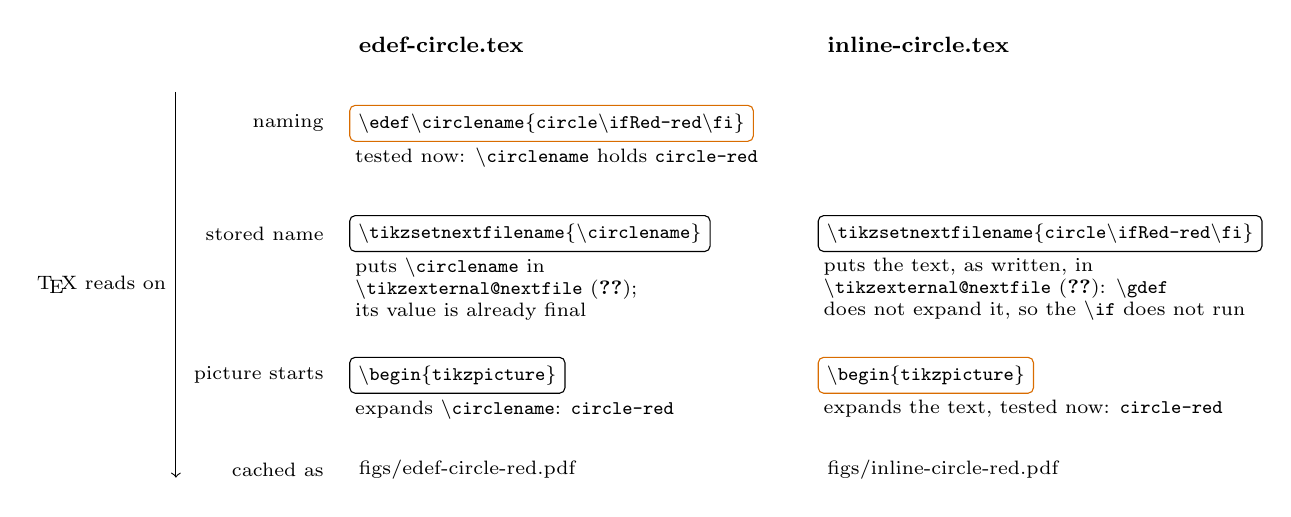
\begin{tikzpicture}[x=1cm, y=-1cm, font=\footnotesize,
    code/.style={draw, rounded corners=2pt, inner sep=3pt, font=\ttfamily\scriptsize, anchor=west},
    test/.style={code, draw=orange!85!black},
    note/.style={font=\scriptsize, anchor=north west, inner sep=2pt},
    stage/.style={font=\scriptsize, anchor=east, align=right}]
  \node[font=\footnotesize\bfseries, anchor=west] at (2.4,0) {\name{edef-circle.tex}};
  \node[font=\footnotesize\bfseries, anchor=west] at (8.35,0) {\name{inline-circle.tex}};
  \draw[->] (0.2,0.6) -- node[left, font=\scriptsize] {\TeX\ reads on} (0.2,5.5);
  % the naming lines
  \node[stage] at (2.2,1) {naming};
  \node[test] (e1) at (2.4,1) {\textbackslash edef\textbackslash circlename\{circle\textbackslash ifRed-red\textbackslash fi\}};
  \node[note] at (e1.south west) {tested now: \cs{circlename} holds \texttt{circle-red}};
  \node[stage] at (2.2,2.4) {stored name};
  \node[code] (e2) at (2.4,2.4) {\textbackslash tikzsetnextfilename\{\textbackslash circlename\}};
  \node[note, align=left] at (e2.south west) {puts \cs{circlename} in\\\cs{tikzexternal@nextfile} (\Cref{sec:override});\\its value is already final};
  \node[code] (i2) at (8.35,2.4) {\textbackslash tikzsetnextfilename\{circle\textbackslash ifRed-red\textbackslash fi\}};
  \node[note, align=left] at (i2.south west) {puts the text, as written, in\\\cs{tikzexternal@nextfile} (\Cref{sec:override}): \cs{gdef}\\does not expand it, so the \cs{if} does not run};
  % the picture starts: TikZ expands the stored name
  \node[stage] at (2.2,4.2) {picture starts};
  \node[code] (e3) at (2.4,4.2) {\textbackslash begin\{tikzpicture\}};
  \node[note] at (e3.south west) {expands \cs{circlename}: \texttt{circle-red}};
  \node[test] (i3) at (8.35,4.2) {\textbackslash begin\{tikzpicture\}};
  \node[note] at (i3.south west) {expands the text, tested now: \texttt{circle-red}};
  \node[stage] at (2.2,5.4) {cached as};
  \node[anchor=west, font=\scriptsize] at (2.4,5.4) {\name{figs/edef-circle-red.pdf}};
  \node[anchor=west, font=\scriptsize] at (8.35,5.4) {\name{figs/inline-circle-red.pdf}};
\end{tikzpicture}
\end{center}

The \cs{edef} form tests the flag on its own line, before \cs{tikzsetnextfilename}; the inline form tests it only when the picture starts. Between the two lines nothing touches the flag, so both tests give \texttt{circle-red}.

We can check what is stored by printing \cs{tikzexternal@nextfile} and \cs{circlename} right before each picture starts, without editing any file:

\begin{pane}
$ hook='\AddToHook{env/tikzpicture/before}{\typeout{NEXTFILE: \expandafter\meaning\csname tikzexternal@nextfile\endcsname}\typeout{CIRCLENAME: \meaning\circlename}}'   # print both macros before each picture
$ for e in inline edef; do pdflatex -shell-escape -interaction=batchmode -jobname $e "$hook\input{$e}"; done   # compile both with the hook
$ grep --extended-regexp '^(NEXTFILE|CIRCLENAME)' inline.log edef.log   # what the hook printed
\end{pane}
\begin{cmdout}
inline.log:NEXTFILE: macro:->circle\ifRed -red\fi
inline.log:CIRCLENAME: undefined
inline.log:NEXTFILE: macro:->circle\ifRed -red\fi
inline.log:CIRCLENAME: undefined
edef.log:NEXTFILE: macro:->\circlename
edef.log:CIRCLENAME: macro:->circle
edef.log:NEXTFILE: macro:->\circlename
edef.log:CIRCLENAME: macro:->circle-red
\end{cmdout}

\begin{itemize}[leftmargin=1.2em,itemsep=0pt]
  \item \verb|\AddToHook{env/tikzpicture/before}{...}| runs its code each time a \texttt{tikzpicture} is about to start, the moment TikZ reads the stored name.
  \item \verb|\typeout| writes to the log; \verb|\meaning| turns a macro's contents into text without running them. \verb|\csname tikzexternal@nextfile\endcsname| spells out the name with its \texttt{@}, which plain document code cannot type directly, and \verb|\expandafter| builds that name before \verb|\meaning| looks at it.
  \item \texttt{-jobname} keeps the experiment's name, so TikZ finds the images it has already cached.
\end{itemize}
Each experiment draws two pictures, plain then red, so each prints two pairs. The inline form stores the same text both times, with the \cs{if} still in it, and \cs{circlename} does not exist. The \cs{edef} form stores \cs{circlename} both times, and \cs{circlename} already holds the finished name: \texttt{circle}, then \texttt{circle-red}.

\begin{insight}{So why the \cs{edef}?}
It is not needed. It freezes the name at the moment you write it, instead of when TikZ gets to it. That only differs if a flag changes between \cs{tikzsetnextfilename} and the \texttt{tikzpicture}, which in our figure files never happens. The inline form is shorter and just as correct.

Neither is needed in the book at all: my chain and override already give each variant its own name. They write every name out in full, which costs a line per variant but keeps each name visible to \name{grep}. Claude's variants save lines by assembling the name from the flags, so no file name appears anywhere in the source.
\end{insight}

\begin{result}{What to do in the book}
Give \name{ambient-space.tex} my override form, like \name{ellipse.tex}: a default name, then one line per flag. Every variant gets its own cached image, and every name can be found with \name{grep}.
\end{result}

\section*{Summary}

\begin{center}\small
\begin{tabular}{@{}lll@{}}
  \toprule
  naming & pictures & cached \\
  \midrule
  one fixed name & wrong: the second reuses the first & yes \\
  \texttt{export next=false} & right & no, redrawn every build \\
  my \cs{if}…\cs{else} chain & right & yes; every name written out \\
  my default plus overrides & right & yes; every name written out \\
  Claude's \cs{edef} name & right & yes; names built from the flags \\
  Claude's inline \cs{if} in the name & right & yes; names built from the flags \\
  \bottomrule
\end{tabular}
\end{center}

\section*{What to read}

From my library, in this order, for what this lesson touches:
\begin{itemize}[leftmargin=1.2em,itemsep=0pt]
  \item \cite{tbt}, ch.~11 \textit{Macros} (pp.~109--124), ch.~12 \textit{Expansion} (pp.~125--139, \cs{edef} in §12.3.2), ch.~13 \textit{Conditionals} (pp.~140--151, \cs{newif} on p.~144).
  \item \cite{feuersanger}, §2.3 \textit{Expansion control} to §2.5 \textit{Branching} (pp.~5--16): the same ground in 12 pages, with pgf's own idioms.
  \item \cite{tikz}, §52.4 \textit{Externalizing graphics} (pp.~670--680): \cs{tikzsetnextfilename}, \texttt{export next}, the MD5 check.
\end{itemize}

\begin{thebibliography}{TeXbyTopic}\raggedright
  \bibitem[TeXbyTopic]{tbt} Victor Eijkhout, \textit{\TeX\ by Topic, a \TeX nician's reference}. \url{https://ctan.org/pkg/texbytopic}
  \bibitem[TeX]{feuersanger} Christian Feuersänger, \textit{Notes on programming in \TeX}, revision 1.18.1, 15 May 2021, shipped with \name{pgfplots} (\texttt{texdoc TeX-programming-notes}). \url{https://ctan.org/pkg/pgfplots}
  \bibitem[TikZ]{tikz} Till Tantau, \textit{The Ti\textit{k}Z and PGF packages}, manual for version 3.1.10. Section 52, \textit{Externalization library}, by Christian Feuersänger. \url{https://ctan.org/pkg/pgf}
\end{thebibliography}

\end{document}
